\documentclass[smallcondensed]{svjour3}                     % onecolumn (standard format)
%\documentclass{article}
\RequirePackage{fix-cm}

\usepackage{graphicx}
\usepackage[fleqn]{amsmath}
\usepackage{amssymb}
\usepackage{bm}
%\usepackage{pgf}
%\usepackage[polutonikogreek]{babel}

\begin{document}

\title{A linearization procedure for constrained multibody systems}

\titlerunning{A linearization procedure for constrained multibody systems}        % if too long for running head

\author{Dale L. Peterson\and Gilbert Gede\and Mont Hubbard}

\institute{Dale L. Peterson, Gilbert Gede, Mont Hubbard \at
           Sports Biomechanics Laboratory\\
           Department of Mechanical and Aerospace Engineering\\
           University of California Davis\\
           Davis, CA 95616-5294\\
           Tel.: +1 530 752 2163\\
           \email{\{dlpeterson,ggede,mhubbard\}@ucdavis.edu}}

\date{Received: date / Accepted: date}

\maketitle

\begin{abstract}
% Context
Many common mechanical systems have configuration or velocity constraints.
% Need  (what we have and what we want)
Analyses of such systems often require linearized forms of the motion
equations.  Although derivation of the nonlinear motion equations is well
understood, very little has been presented on the proper approach to
forming linearized versions which satisfy the constraints.
% Task
To address this issue, we developed a procedure for organizing the constraints
and motion equations, and subsequently linearizing these equations.
% Object of the document
In this paper we present this procedure to linearize the nonlinear motion
equations of constrained multibody systems, and illustrate it with a familiar
example, the rolling disc.
% Findings
We apply this procedure to a model of a bicycle that includes a closed
kinematic loop and four nonholonomic constraints and find that the resulting
symbolic linearized motion equations are identical to previously published
results.  The technique can be performed symbolically (enabling explicit
analytical forms of the linearized dynamics) or numerically.
% Conclusion
Motion equations for constrained multibody systems can now be linearized in a
systematic fashion, symbolically or numerically, thereby facilitating common
linear analyses (e.g., stability analysis and control system design).
% Perspectives
Efficiency of computer implementations of this procedure will be considered in
future studies.
\keywords{linearization, constrained multibody systems, symbolic dynamics, control}
\end{abstract}

%In summary, the procedure is:
%\begin{enumerate}
%    \item Describe the system in the form of the equations shown in Table
%        \ref{table:assumptions}.
%    \item Determine a point of linearization ($\bm{q}^*$, $\dot{\bm{q}}^*$,
%      $\bm{u}^*$, $\dot{\bm{u}}^*$, and $\bm{r}^*$) which satisfies the
%      equations in Table \ref{table:assumptions}.
%    \item Compute the quantities in equation (\ref{eq:quant_to_compute}).
%    \item Identify independent coordinates and speeds; form equations (\ref{eq:C_0}), (\ref{eq:C_1}), and
%        (\ref{eq:C_2}).
%    \item Form equation (\ref{eq:state_space_constrained}), and if needed,
%      equations (\ref{eq:A_prime})-(\ref{eq:B}).
%\end{enumerate}

\section{Introduction}
\label{sec:intro}
Multibody systems, rigid or flexible, and particles often have constraints
which limit how they can move. In this paper, we will discuss 3 types of
constraints: configuration, velocity, and acceleration. Configuration
constraints limit the location or orientation of parts of the system, relative
to the external world or other parts of the system. Velocity constraints limit
the speeds at which the configuration can change, either from configuration
constraints (through time differentiation) or independent application. In this
paper, acceleration constraints refer to time differentiated velocity
constraints. Examples of multibody systems with constraints include closed
kinematic loops or objects rolling without slip.

Linear equations of motion are necessary for many different analyses.
Stability analysis and control system design are two possible scenarios.
Linearization of these constrained systems is not straightforward and presents
significant challenges. Computing the Jacobian matrix of the differential
equations - without considering the system's constraints - will give incorrect
results.

Currently, only a few approaches to linearizing constrained systems which have
been presented\cite{Kang2003}, \cite{Negrut2006}. A limitation of these
approaches is that they have been developed for equations of motion found using
Lagrange's method, which contain Lagrange multipliers. Kane's method
\cite{Kane1985} allows formulation of equations of motion for constrained
systems in which no multipliers are present. The dynamics of these systems can
be completely described by ordinary differential equations. This significantly
different formulation requires a different approach to linearization than what
existing options provide.

The goal of this paper is to establish concretely the first order relationships
(about an arbitrary point of linearization) between a selection of independent
coordinates and speeds and the time-derivatives of all coordinates and speeds
(both independent and dependent). The formalism presented here is generic
enough to cover most examples of time-varying constrained multibody systems
with arbitrary external inputs and arbitrary specified quantities.  The
procedure was created for systems whose equations of motion have been derived
with Kane's method. Although also applicable to dynamic system equations
formulated using other methods, it is restricted to systems which can be
completely described by a set of ODEs (i.e., DAEs needn't be solved).

We first present the linearization procedure, followed by some discussion of
the procedure, together with an example. The derivation of the procedure is
provided in Section \ref{sec:derivations}. Additionally, the electronic
supplementary material provides more examples (in more detail) and an
alternative ordering for the independent/dependent quantities.

%The complete configuration of the system is further assumed to be described by
%generalized coordinates $\bm{q}\in\bm{R}^n$ and its velocity completely
%described by generalized speeds $\bm{u}\in\bm{R}^o$, with $n \ne o$ in general.
%All coordinates and speeds, not only the independent ones, are represented by
%$\bm{q}$ and $\bm{u}$.  The system is assumed to be governed by the
%relationships described in Table \ref{table:assumptions}.  The system is
%described by $l + m + n + o$ equations which relate $2n + 2o + s + 1$
%quantities, which implies that $n - l + o - m + s + 1$ of these quantities are
%independent.  This paper discusses the first order relationship between these
%independent quantities ($n-l$ independent coordinates, $o-m$ independent
%speeds, $s$ control inputs, and time $t$) and the time derivatives of the $n$
%coordinates and $o$ speeds.
%
%The first three equations in Table \ref{table:assumptions} represent
%constraints derived purely from kinematic considerations at the configuration,
%velocity, and acceleration levels, respectively.  The velocity constraints may
%be nonholonomic or time differentiated holonomic.  The acceleration constraints
%can be time differentiated velocity constraints or kinematic acceleration
%constraints.  The fourth equation represents kinematic differential equations
%which relate $\bm{\dot{q}}$ to $\bm{u}$ and are linear in both these
%quantities.  The fifth equation represents the constraint-free nonholonomic
%dynamic differential equations~\cite{Kane1985}, and will necessarily be linear
%in $\bm{\dot{u}}$ and the inputs $\bm{r}$, but generally nonlinear in all other
%quantities.  This formalism is exceedingly generic; in practice, the structure
%of the functions in Table \ref{table:assumptions} can be leveraged to simplify
%the following calculations.  This will be discussed subsequently.
%
%Trajectories of the system exist on a $p \triangleq n - l + o - m$ dimensional
%manifold embedded in a $n + o$ dimensional space, though conserved quantities
%(e.g., total mechanical energy) may restrict trajectories to a lower
%dimensional manifold.  In general this cannot be assumed, however, especially
%in the presence of exogenous inputs $\bm{r}$ which may change the total
%mechanical energy of the system.  While more than $p$ of the independent state
%variables may be of interest (i.e., dependent coordinates or speeds may be of
%interest in themselves), only $p$ quantities are truly independent.  Which of
%these $p$ coordinates and speeds should be chosen as independent out of the
%possible $n + o$ may be obvious for small systems where there is intuition
%about system behavior, but in general the optimal choice depends on how the
%configuration $\bm{q}$ affects the gradients of $f_c$ and $f_v$.  On the other
%hand, in systems with cyclic (ignorable) coordinates, fewer than $p$ state
%variables may be of interest; one example is the Whipple bicycle model where
%$p=10$ but 5 of these state variables are cyclic coordinates (Cartesian
%coordinates of rear wheel contact point, heading, and both wheel angles) and
%may only be of secondary interest.

\section{Results}
\label{sec:results}
The linearized equations of motion are
\begin{align}
  \label{eq:state_space_constrained}
  \left[
    \begin{array}{cc}
      \tilde{M}_{qq} & \bm{0}_{n \times o} \\
      \tilde{M}_{uqc} & \tilde{M}_{uuc} \\
      \tilde{M}_{uqd} & \tilde{M}_{uud}
    \end{array}
    \right]
    \left[
      \begin{array}{c}
        \delta \bm{\dot{q}} \\
        \delta \bm{\dot{u}}
      \end{array}
    \right]
   &=
   \left[
     \begin{array}{cc}
       (\tilde{A}_{qq} + \tilde{A}_{qu} C_1 ) C_0 & \tilde{A}_{qu} C_2 \\
       (\tilde{A}_{uqc} + \tilde{A}_{uuc} C_1 ) C_0 & \tilde{A}_{uuc} C_2\\
       (\tilde{A}_{uqd} + \tilde{A}_{uud} C_1 ) C_0 & \tilde{A}_{uud} C_2
     \end{array}
   \right]
    \left[
      \begin{array}{c}
        \delta \bm{q}_i \\
        \delta \bm{u}_i
      \end{array}
    \right]
    +
    \left[
      \begin{array}{c}
        \bm{0}_{(n+m) \times s} \\
        \tilde{B}_{u}
      \end{array}
    \right]
    \delta \bm{r}
\end{align}
Table \ref{table:assumptions} provides the form in which the nonlinear
equations of motion and constraints must be arranged in order to carry out the
linearization procedure.  Equations (\ref{eq:quant_to_compute}) provides the
bulk of the terms in equation (\ref{eq:state_space_constrained}); these terms
are Jacobian matrices of the differential equations. Equations
(\ref{eq:C_0})-(\ref{eq:C_2}) provide the terms $C_0$, $C_1$, and $C_2$ which
embed the constraints into (\ref{eq:state_space_constrained}). Finally, the
permutation matrices in equations (\ref{eq:Pq}) and (\ref{eq:Pu}) separate the
independent and dependent speeds.

\begin{table}[htbp]
  \centering
  \caption{Constrained multibody system governing definitions and equations}
  \label{table:assumptions}
  \begin{tabular}[c]{l l l}
    Quantity & Shape & Description\\
    \hline
    $\bm{q},\bm{\dot{q}}$ & $\mathbf{R}^n$ & Coordinates and their time
    derivatives\\
    $\bm{u}, \bm{\dot{u}}$ & $\mathbf{R}^o$ & Speeds and their time derivatives\\
    $\bm{r}$ & $\mathbf{R}^s$ & Exogenous inputs \\
  \end{tabular}
  \begin{tabular}[c]{r @{ $=$ } l l}
    \multicolumn{3}{c}{ } \\
    \multicolumn{2}{c}{Equation} & Description \\
    \hline
    $\bm{f}_{c}(\bm{q}, t)$ & $\bm{0}_{l \times 1}$ & Configuration constraints \\
    $\bm{f}_{v}(\bm{q}, \bm{u}, t)$ & $\bm{0}_{m \times 1}$ & Velocity constraints \\
    $\bm{f}_{a}(\bm{q}, \bm{\dot{q}}, \bm{u}, \bm{\dot{u}}, t)$ & $\bm{0}_{m
    \times 1}$ & Acceleration constraints \\
    $\bm{f}_{0}(\bm{q}, \bm{\dot{q}}, t) + \bm{f}_{1}(\bm{q}, \bm{u}, t)$ &
    $\bm{0}_{n \times 1}$ & Kinematic differential equations \\
    $\bm{f}_{2}(\bm{q}, \bm{\dot{u}}, t) + \bm{f}_{3}(\bm{q}, \bm{\dot{q}},
    \bm{u}, \bm{r}, t)$ & $\bm{0}_{(o - m) \times 1}$ & Dynamic differential equations
  \end{tabular}
\end{table}

The matrices in (\ref{eq:state_space_constrained}) are evaluated at the point
of linearization $\bm{q}=\bm{q}^*, \bm{\dot{q}}=\bm{\dot{q}}^*,
\bm{u}=\bm{u}^*, \bm{\dot{u}}=\bm{\dot{u}}^*, \bm{r}=\bm{r}^*$; this point must
satisfy the equations in Table \ref{table:assumptions}, and may or may not be
an equilibrium point.


\begin{align}
\label{eq:quant_to_compute}
  \begin{array}{llcll}
    \tilde{M}_{qq}  &\triangleq \nabla_{\bm{\dot{q}}}\bm{f}_0 & \quad &
    \tilde{M}_{uqc} &\triangleq \nabla_{\bm{\dot{q}}}\bm{f}_a \\
    \tilde{M}_{uuc} &\triangleq \nabla_{\bm{\dot{u}}}\bm{f}_a & \quad &
    \tilde{M}_{uqd} &\triangleq \nabla_{\bm{\dot{q}}}\bm{f}_3 \\
    \tilde{M}_{uud} &\triangleq \nabla_{\bm{\dot{u}}}\bm{f}_2 & \quad &
    \tilde{A}_{qq}  &\triangleq -\nabla_{\bm{q}}(\bm{f}_0 + \bm{f}_1) \\
    \tilde{A}_{qu}  &\triangleq -\nabla_{\bm{u}}\bm{f}_1 & \quad &
    \tilde{A}_{uqc} &\triangleq - \nabla_{\bm{q}} \bm{f}_a \\
    \tilde{A}_{uuc} &\triangleq - \nabla_{\bm{u}} \bm{f}_a & \quad &
    \tilde{A}_{uqd} &\triangleq - \nabla_{\bm{q}} (\bm{f}_2 + \bm{f}_3) \\
    \tilde{A}_{uud} &\triangleq - \nabla_{\bm{u}} \bm{f}_3 & \quad &
    \tilde{B}_{u}   &\triangleq -\nabla_{\bm{r}}\bm{f}_{3}
  \end{array}
\end{align}

\begin{align}
  \label{eq:C_0}
  C_0 &\triangleq \left[ I_{n \times n} - P_{qd}(\nabla_{\bm{q}}
    \bm{f}_{c} P_{qd})^{-1} \nabla_{\bm{q}} \bm{f}_{c} \right] P_{qi}\\
  \label{eq:C_1}
  C_1 &\triangleq -P_{ud}(\nabla_{\bm{u}} \bm{f}_{v} P_{ud})^{-1}
  \nabla_{\bm{q}} \bm{f}_{v} \\
  \label{eq:C_2}
  C_2 &\triangleq \left[I - P_{ud} (\nabla_{\bm{u}}\bm{f}_{v} P_{ud})^{-1} \nabla_{\bm{u}}
    \bm{f}_{v} \right] P_{ui}\\
  \label{eq:Pq}
  \bm{q} &= P_{qi} \bm{q}_{i} + P_{qd} \bm{q}_{d} \\
  \label{eq:Pu}
  \bm{u} &= P_{ui} \bm{u}_{i} + P_{ud} \bm{u}_{d}
\end{align}

\section{Discussion}
\label{sec:discussion}
Equation (\ref{eq:state_space_constrained}) doesn't fit into the standard linear
system framework because it is non-square.  To obtain a square system (useful
in stability analysis and control system design) we define
\begin{align}
  \label{eq:A_prime}
    A^\prime &\triangleq \tilde{M}^{-1} \tilde{A} \\
  \label{eq:B_prime}
    B^\prime &\triangleq \tilde{M}^{-1} \tilde{B}
\end{align}
where  $A^\prime \in \bm{R}^{(o + n) \times (o - m + n -l)}$, $B^\prime \in
\bm{R}^{(o + n) \times s}$.  We can extract the rows corresponding to the
independent states by defining
\begin{align}
  \label{eq:P_prime}
    P^\prime &\triangleq \begin{bmatrix}
        P_{qi} & \bm{O}_{n \times (o - m)} \\
        \bm{O}_{o \times (n - l)} & P_{ui}
    \end{bmatrix} \\
  \label{eq:A}
    A &\triangleq P^{\prime T} A^\prime \\
  \label{eq:B}
    B &\triangleq P^{\prime T} B^\prime
\end{align}
where $P^\prime \in \bm{R}^{(o - m + n - l) \times (o - m + n - l)}$.  Defining
$\bm{x}_i = \left[\delta\bm{q}_i,\,\delta\bm{u}_i\right]^{T}$ yields the square
state space system $\dot{\bm{x}}_i = A \bm{x}_i + B \bm{r}$ to which standard
linear systems analyses may applied.  It is worth noting that the rows
of $A^\prime$ and $B^\prime$ which correspond to dependent states can be used
in the output or measurement equations of a linear state space model, as in the
case when the controlling or measuring dependent state(s).

The choice of which state variables are taken to be independent may determine
whether $\nabla_{\bm{q}}\bm{f}_{c} P_{qd}$ and $\nabla_{\bm{u}} \bm{f}_{v}
P_{ud}$ are nonsingular.  These matrices depend upon the configuration $\bm{q}$
and constant parameters; for certain configurations or parameters, it may be
that the choice of independent state variables cannot be arbitrary.  While some
systems may permit a choice of independent state variables which are valid for
all configurations of interest, others may not.  Methods for automatically
selecting the ``best'' choice of independent state variables are discussed in
\cite{Reckdahl1996}; they involve computing the SVD of the Jacobian of the
constraint matrices to determine a set of independent speeds which will ensure
the non-singularity of the aforementioned matrices.

This algorithm as been applied to two well studied systems: the rolling disc
and an extended version of the Whipple bicycle model\cite{Meijaard2007}.
Detailed model description, derivation, and benchmarking results are presented
in the electronic supplementary material.

\section{Example}
\label{example}
We apply this linearization technique to the well studied rolling disc.  Figure
\ref{fig:disc} illustrates the choice of coordinates, speeds, and parameters.
The disc is assumed to be knife edged of radius $r$, mass $m$, spin inertia
$J$, and transverse inertia $I$.  To illustrate the concept of dependent
quantities, we purposefully choose to describe the configuration and velocity
of the disc with a non-minimal set of coordinates and speeds.  This choice is
not purely academic.  It is convenient for a physical disc equipped with a rate
gyroscope and accelerometer to measure these body fixed quantities (or their
time derivatives) directly, rather than the more traditional set which is
chosen for analytic convenience.  In more complicated systems with constraints,
it is difficult (if not impossible) to describe the system with a minimal
choice of coordinates and speeds; the ideas demonstrated by this simple example
can be applied to more complicated ones.

The orientation of the disc-fixed frame $C$ relative to the inertial frame $N$
is given by a sequence of angular rotations (Euler ZXY) through angles $q_0$
(yaw), $q_1$ (lean), and $q_2$ (spin).  The angular velocity of $C$ in $N$, the
location of disc center $C^*$ relative to the inertial origin $N^*$, and the
velocity of $C^*$ in $N$ are
\begin{align}
  \bm{\omega}^C &= u_0 \bm{c}_x + u_1 \bm{c}_y + u_2 \bm{c}_z \\
  \bm{r}^{C^*} &= q_3 \bm{n}_x + q_4 \bm{n}_y + q_5 \bm{n}_z \\
  \bm{v}^{C^*} &= u_3 \bm{c}_x + u_4 \bm{c}_y + u_5 \bm{c}_z
\end{align}
If the disc is in contact with the ground, a configuration constraint involving
the height $q_5$ of the disc center and the lean $q_1$.  Similarly, if the disc
rolls without slip, other constraints relate the generalized speeds $u_i, (i =
0,\dots,5)$.  The derivations of these constraints and the equations of motion
are presented in the electronic supplementary material and can also be found in
the literature \cite{O'Reilly1996}.
\begin{table}[htbp]
  \centering
  \caption{Rolling disc governing definitions and equations}
  \label{table:rollingdisc}
  \begin{tabular}[c]{l l l}
    Quantity & Shape & Description\\
    \hline
    $\bm{q},\bm{\dot{q}}$ & $\mathbf{R}^6$ & Coordinates and their time
    derivatives\\
    $\bm{u}, \bm{\dot{u}}$ & $\mathbf{R}^6$ & Speeds and their time derivatives
  \end{tabular}
  \begin{tabular}[c]{r @{ $=$ } l}
%    \multicolumn{3}{c}{ } \\
%    \multicolumn{2}{c}{Equation} &           \\
    \hline
    % Configuration constraint
    $\bm{f}_c$ & $rc_1 + q_5$ \\
    % Velocity constraints
    $\bm{f}_v$ & $\left[\begin{array}{c}
        r u_1 c_2 + u_3 \\
        -r (u_0 c_2 + u_2 s_2) + u_4 \\
        r u_1 s_2 + u_5
    \end{array}\right] $ \\
    % Acceleration constraints
    $\bm{f}_a$ & $\left[\begin{array}{c}
        -r (u_1 \dot{q}_2 s_2 + \dot{u}_1 c_2) + \dot{u}_3 \\
        -r ((\dot{u}_2 - u_0 \dot{q}_2) s_2   + (\dot{u}_0 + u_2 \dot{q}_2)c_2) + \dot{u}_4 \\
      r (u_1 \dot{q}_2 c_2 + s_2 \dot{u}_1) + \dot{u}_5
      \end{array}\right]$ \\
    % Kinematic differential equations
    $\bm{f}_0$ &
        $\left[\begin{array}{c}
-\dot{q}_0 s_2 c_1 + \dot{q}_1 c_2 \\
\dot{q}_0 s_1 + \dot{q}_2 \\
\dot{q}_0 c_1 c_2 + \dot{q}_1 s_2 \\
\dot{q}_3 (-s_0 s_1 s_2 + c_0 c_2)
+ \dot{q}_4 (s_0 c_2 + s_1 s_2 c_0)
- \dot{q}_5 s_2 c_1\\
- \dot{q}_3 s_0 c_1 + \dot{q}_4 c_0 c_1 + \dot{q}_5 s_1 \\
\dot{q}_3 (s_0s_1c_2 + s_2c_0) + \dot{q}_4 (s_0s_2 - s_1c_0c_2) + \dot{q}_5 c_1 c_2
         \end{array}\right]$ \\
    $\bm{f}_1$ & $\left[\begin{array}{c}-u_0 \\ -u_1 \\ -u_2 \\
             -u_3 \\ -u_4 \\ -u_5 \end{array}\right]$ \\
    % Dynamic differential equations
  $\bm{f}_2$ & $\left[\begin{array}{c}
-I \dot{u}_0 - m r c_2 \dot{u}_4 \\
-J \dot{u}_1 + m r s_2 \dot{u}_5 + m r c_2 \dot{u}_3 \\
-I \dot{u}_2 - m r s_2 \dot{u}_4
                   \end{array}\right]$ \\

  $\bm{f}_3$ & $\left[\begin{array}{c}
-I u_1 u_2 + J u_1 u_2 + g m r s_1 c_2 - m r (-u_0 u_5 + u_2 u_3) c_2 \\
                m r (u_0 u_4 - u_1 u_3) s_2 + m r (u_1 u_5 - u_2 u_4) c_2 \\
 I u_0 u_1 - J u_0 u_1 + g m r s_1 s_2 - m r (-u_0 u_5 + u_2 u_3) s_2
                   \end{array}\right]$
  \end{tabular}
\end{table}

%f_c:
%[r*cos(q1) + q5]
%f_v:
%[                r*u1*cos(q2) + u3]
%[-r*(u0*cos(q2) + u2*sin(q2)) + u4]
%[                r*u1*sin(q2) + u5]
%f_a:
%[                                -r*u1*sin(q2)*q2' + r*cos(q2)*u1' + u3']
%[-r*(-u0*sin(q2)*q2' + u2*cos(q2)*q2' + sin(q2)*u2' + cos(q2)*u0') + u4']
%[                                 r*u1*cos(q2)*q2' + r*sin(q2)*u1' + u5']
%f_0:
%[                                                                                      -sin(q2)*cos(q1)*q0' + cos(q2)*q1']
%[                                                                                                       sin(q1)*q0' + q2']
%[                                                                                       sin(q2)*q1' + cos(q1)*cos(q2)*q0']
%[(sin(q0)*cos(q2) + sin(q1)*sin(q2)*cos(q0))*q4' + (-sin(q0)*sin(q1)*sin(q2) + cos(q0)*cos(q2))*q3' - sin(q2)*cos(q1)*q5']
%[                                                                -sin(q0)*cos(q1)*q3' + sin(q1)*q5' + cos(q0)*cos(q1)*q4']
%[ (sin(q0)*sin(q2) - sin(q1)*cos(q0)*cos(q2))*q4' + (sin(q0)*sin(q1)*cos(q2) + sin(q2)*cos(q0))*q3' + cos(q1)*cos(q2)*q5']
%f_1:
%[-u0]
%[-u1]
%[-u2]
%[-u3]
%[-u4]
%[-u5]
%f_2:
%[                  -I*u0' - m*r*cos(q2)*u4']
%[-J*u1' + m*r*sin(q2)*u5' + m*r*cos(q2)*u3']
%[                  -I*u2' - m*r*sin(q2)*u4']
%f_3:
%[-I*u1*u2 + J*u1*u2 + g*m*r*sin(q1)*cos(q2) - m*r*(-u0*u5 + u2*u3)*cos(q2)]
%[                m*r*(u0*u4 - u1*u3)*sin(q2) + m*r*(u1*u5 - u2*u4)*cos(q2)]
%[ I*u0*u1 - J*u0*u1 + g*m*r*sin(q1)*sin(q2) - m*r*(-u0*u5 + u2*u3)*sin(q2)]

\begin{figure}
  \centering
  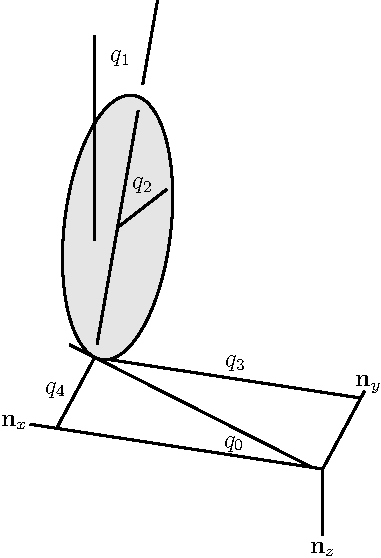
\includegraphics{rollingdisc.pdf}
  \caption{Rolling disc configuration}
  \label{fig:disc}
\end{figure}

The matrices which make up the linear equations were created using the method
presented in Section \ref{sec:results}. It is important to note that the
entries in these matrices must be evaluated at the point of linearization
($\bm{q}^*, \bm{\dot{q}}^*, \bm{u}^*, \bm{\dot{u}}^*$), and that this point of
linearization must satisfy the equations in Table \ref{table:assumptions}.
There is no requirement that this point be an equilibrium point, which implies
that in general both $\bm{\dot{q}}$ and $\bm{\dot{u}}$ may be non-zero. To
reduce the complexity of the equations, we chose $q_0^* = q_2^* = 0$.  This
means that the other quantities in the linearized equations (other $q$'s, the
$\dot{q}$'s, the $u$'s, and the $\dot{u}$'s) need to be solved for with these 2
quantities already set to 0.

The independent state vector is:
\begin{align}
\begin{bmatrix}
\delta \bm{q}_i \\
\delta \bm{u}_i
\end{bmatrix} =
\begin{bmatrix}
q_0 &
q_1 &
q_2 &
q_3 &
q_4 &
u_0 &
u_1 &
u_2
\end{bmatrix}^T
\end{align}

And the complete (independent and dependent) state vector is:
\begin{align}
\begin{bmatrix}
\delta \bm{q} \\
\delta \bm{u}
\end{bmatrix} =
\left[
\begin{array}{cccccccccccc}
q_0 &
q_1 &
q_2 &
q_3 &
q_4 &
q_5 &
u_0 &
u_1 &
u_2 &
u_3 &
u_4 &
u_5
\end{array}
\right]^T
\end{align}

The coefficient matrices of the linearized equations (Equation
\ref{eq:state_space_constrained}) are:
\begin{equation}
  \left[
    \begin{array}{cc}
      \tilde{M}_{qq} & \bm{0}_{n \times o} \\
      \tilde{M}_{uqc} & \tilde{M}_{uuc} \\
      \tilde{M}_{uqd} & \tilde{M}_{uud}
    \end{array}
    \right]=
\left[\begin{smallmatrix}0 & 1 & 0 & 0 & 0 & 0 & 0 & 0 & 0 & 0 & 0 & 0\\s_{1} & 0 & 1 & 0 & 0 & 0 & 0 & 0 & 0 & 0 & 0 & 0\\c_{1} & 0 & 0 & 0 & 0 & 0 & 0 & 0 & 0 & 0 & 0 & 0\\0 & 0 & 0 & 1 & 0 & 0 & 0 & 0 & 0 & 0 & 0 & 0\\0 & 0 & 0 & 0 & c_{1} & s_{1} & 0 & 0 & 0 & 0 & 0 & 0\\0 & 0 & 0 & 0 & - s_{1} & c_{1} & 0 & 0 & 0 & 0 & 0 & 0\\0 & 0 & 0 & 0 & 0 & 0 & 0 & r & 0 & 1 & 0 & 0\\0 & 0 & - r u_{2} & 0 & 0 & 0 & - r & 0 & 0 & 0 & 1 & 0\\0 & 0 & r u_{1} & 0 & 0 & 0 & 0 & 0 & 0 & 0 & 0 & 1\\0 & 0 & 0 & 0 & 0 & 0 & - \frac{1}{4} m r^{2} & 0 & 0 & 0 & - m r & 0\\0 & 0 & 0 & 0 & 0 & 0 & 0 & - \frac{1}{2} m r^{2} & 0 & m r & 0 & 0\\0 & 0 & 0 & 0 & 0 & 0 & 0 & 0 & - \frac{1}{4} m r^{2} & 0 & 0 & 0\end{smallmatrix}\right]
\end{equation}


\begin{equation*}
   \left[
     \begin{array}{cc}
       (\tilde{A}_{qq} + \tilde{A}_{qu} C_1 ) C_0 & \tilde{A}_{qu} C_2 \\
       (\tilde{A}_{uqc} + \tilde{A}_{uuc} C_1 ) C_0 & \tilde{A}_{uuc} C_2\\
       (\tilde{A}_{uqd} + \tilde{A}_{uud} C_1 ) C_0 & \tilde{A}_{uud} C_2
     \end{array}
   \right]=
\end{equation*}
\begin{equation}
\left[\begin{smallmatrix}0 & 0 & c_{1} \dot{q}_{0} & 0 & 0 & 1 & 0 & 0\\0 & - c_{1} \dot{q}_{0} & 0 & 0 & 0 & 0 & 1 & 0\\0 & s_{1} \dot{q}_{0} & - \dot{q}_{1} & 0 & 0 & 0 & 0 & 1\\- \dot{q}_{4} & 0 & c_{1} \dot{q}_{5} - s_{1} \dot{q}_{4} & 0 & 0 & 0 & - r & 0\\c_{1} \dot{q}_{3} & - c_{1} \dot{q}_{5} + s_{1} \dot{q}_{4} & r u_{2} & 0 & 0 & r & 0 & 0\\- s_{1} \dot{q}_{3} & c_{1} \dot{q}_{4} + s_{1} \dot{q}_{5} & - r u_{1} - \dot{q}_{3} & 0 & 0 & 0 & 0 & 0\\0 & 0 & r u_{1} \dot{q}_{2} & 0 & 0 & 0 & 0 & 0\\0 & 0 & - r u_{0} \dot{q}_{2} & 0 & 0 & 0 & 0 & r \dot{q}_{2}\\0 & 0 & 0 & 0 & 0 & 0 & - r \dot{q}_{2} & 0\\0 & - c_{1} g m r & m r^{2} u_{0} u_{1} & 0 & 0 & - m r u_{5} & - \frac{5}{4} m r^{2} u_{2} & \frac{1}{4} m r \left(- r u_{1} + 4 u_{3}\right)\\0 & 0 & m r \left(r u_{1} + r u_{2} - u_{0} u_{4} + u_{1} u_{3} - \dot{u}_{5}\right) & 0 & 0 & m r^{2} u_{2} & - m r u_{5} & m r u_{4}\\0 & 0 & m r \left(- g s_{1} - u_{0} u_{5} + u_{2} u_{3} + \dot{u}_{4}\right) & 0 & 0 & \frac{1}{4} m r^{2} u_{1} & \frac{1}{4} m r^{2} u_{0} & 0\end{smallmatrix}\right]
\end{equation}

With this example, we have used our linearization procedure to find linear
equations of motion which respect the system's constraints. Parametric
stability analysis (eigenvalue analysis) can now be performed on these
equations.  These computations were implemented symbolically with the open
source symbolic manipulator SymPy \cite{SymPy2012}.

\section{Conclusions}
A procedure for forming linearized equations of motion for constrained
multi-body systems has been presented.  This procedure can be implemented
symbolically or numerically, and handles configuration, velocity, and
acceleration level constraints.  The procedure has been implemented
symbolically in the \texttt{sympy.physics.mechanics} sub-module of the open
source symbolic manipulator SymPy\cite{SymPy2012}.

\begin{acknowledgements}
 This material is based upon work partially supported by the National Science
 Foundation under award 0928339 and three Google Summer of Code projects (2009,
 2011, 2012).  Jason Moore, Thomas Johnston, Evan Sperber, and Andrew Kickertz
 provided valuable feedback during discussions of multibody dynamics and
 control.
\end{acknowledgements}

\appendix
\section{Derivation of linearization procedure}
\label{sec:derivations}

This appendix outlines the derivation of Equation
(\ref{eq:state_space_constrained}. This equation can be used for simulation,
stability analysis, or it can be reformulated into the traditional state space
equations for a variety of tasks; these topics are discussed in Section
\ref{sec:discussion}.

We begin with a first order Taylor series expansion of the equations in Table
\ref{table:assumptions} about $\bm{q}=\bm{q}^*$, $\bm{\dot{q}}=\bm{\dot{q}}^*$,
$\bm{u}=\bm{u}^*$, $\bm{\dot{u}}=\bm{\dot{u}}^*$, $\bm{r}=\bm{r}^*$; it is
assumed that all of the equations in Table \ref{table:assumptions} are
satisfied by these quantities.  In the interest of brevity, we omit writing
this point of linearization in each gradient in the calculations below; all are
evaluated at this point.  Expansion of the three constraint
equations, keeping only first order terms, yields
\begin{align}
  \label{eq:configuration_expansion}
  \bm{f}_{c}(\bm{q}, t) &\approx \underbrace{\bm{f}_{c}(\bm{q}^*, t)}_{\bm{0}} +
  \nabla_{\bm{q}}\bm{f}_{c} \delta \bm{q}\\
  \label{eq:velocity_expansion}
  \bm{f}_{v}(\bm{q}, \bm{u}, t) &\approx \underbrace{\bm{f}_{v}(\bm{q}^*,
  \bm{u}^*, t)}_{\bm{0}} +  \nabla_{\bm{q}}\bm{f}_{v} \delta \bm{q} +
  \nabla_{\bm{u}}\bm{f}_{v} \delta \bm{u} \\
  \label{eq:acceleration_expansion}
  \bm{f}_{a}(\bm{q}, \bm{\dot{q}}, \bm{u}, \bm{\dot{u}}, t) &\approx
  \underbrace{\bm{f}_{a}(\bm{q}^*, \bm{\dot{q}}^*, \bm{u}^*, \bm{\dot{u}}^*,
t)}_{\bm{0}} +  \nabla_{\bm{q}}\bm{f}_{a} \delta \bm{q} +
\nabla_{\bm{\dot{q}}}\bm{f}_{a}
 \delta \bm{\dot{q}} \notag\\
&+ \nabla_{\bm{u}}\bm{f}_{a} \delta \bm{u} + \nabla_{\bm{\dot{u}}}\bm{f}_{a}
\delta \bm{\dot{u}}
\end{align}
The first terms are identically zero because of the assumption that the
point of linearization satisfies the constraints.  The Taylor series expansion
of the kinematic differential equations is
\begin{align}
  \label{eq:f0_expansion}
  \bm{f}_{0}(\bm{q}, \bm{\dot{q}}, t) &\approx \bm{f}_{0}(\bm{q}^*,
  \bm{\dot{q}}^*, t) + \nabla_{\bm{q}}\bm{f}_{0} \delta\bm{q} +
  \nabla_{\bm{\dot{q}}}\bm{f}_{0} \delta\bm{\dot{q}}\\
  \label{eq:f1_expansion}
  \bm{f}_{1}(\bm{q}, \bm{u}, t) &\approx \bm{f}_{1}(\bm{q}^*,
  \bm{u}^*, t) + \nabla_{\bm{q}}\bm{f}_{1} \delta\bm{q} +
  \nabla_{\bm{u}}\bm{f}_{1} \delta\bm{u}
\end{align}
Summing (\ref{eq:f0_expansion}) and (\ref{eq:f1_expansion}) and recognizing
that the sum of the first term on the right hand side of each equation must
equal zero, we obtain
\begin{align}
  \label{eq:f0_plus_f1_expansion}
  \bm{f}_{0}(\bm{q}, \bm{\dot{q}}, t) + \bm{f}_{1}(\bm{q}, \bm{u}, t) &\approx
  \nabla_{\bm{q}}(\bm{f}_{0} + \bm{f}_{1}) \delta\bm{q} +
  \nabla_{\bm{\dot{q}}}\bm{f}_{0} \delta\bm{\dot{q}} +
  \nabla_{\bm{u}}\bm{f}_{1} \delta\bm{u}
\end{align}
Similarly, a Taylor series expansion of the dynamic differential equations, we
obtain
\begin{align}
  \label{eq:f2_expansion}
  \bm{f}_{2}(\bm{q}, \bm{\dot{u}}, t) &\approx
      \bm{f}_{2}(\bm{q}^*, \bm{\dot{u}}^*, t) +
      \nabla_{\bm{q}}\bm{f}_{2} \delta\bm{q}
      + \nabla_{\bm{\dot{u}}}\bm{f}_{2} \delta\bm{\dot{u}}\\
  \bm{f}_{3}(\bm{q}, \bm{\dot{q}}, \bm{u}, \bm{r}, t) &\approx
  \bm{f}_{3}(\bm{q}^*, \bm{\dot{q}}^*, \bm{u}^*, \bm{r}^*, t) +
  \nabla_{\bm{q}}\bm{f}_{3} \delta\bm{q}\notag\\
  \label{eq:f3_expansion}
  &+ \nabla_{\bm{\dot{q}}}\bm{f}_{3} \delta\bm{\dot{q}}
  + \nabla_{\bm{u}}\bm{f}_{3} \delta \bm{u}
  + \nabla_{\bm{r}}\bm{f}_{3} \delta\bm{r}
\end{align}
Summing (\ref{eq:f2_expansion}) and (\ref{eq:f3_expansion}) and recognizing
that the sum of the first term on the right hand sides of these equations must
equal zero, we obtain
\begin{align}
  \bm{f}_{2}(\bm{q}, \bm{\dot{u}}, t) + \bm{f}_{3}(\bm{q}, \bm{\dot{q}},
  \bm{u}, \bm{r}, t) &\approx \nabla_{\bm{q}}(\bm{f}_2 + \bm{f}_3)
  \delta\bm{q} + \nabla_{\bm{\dot{q}}}\bm{f}_{3} \delta\bm{\dot{q}}\notag\\
  \label{eq:f2_plus_f3_expansion}
  &+ \nabla_{\bm{u}}\bm{f}_{3} \delta\bm{u} +
  \nabla_{\bm{\dot{u}}}\bm{f}_{2} \delta\bm{\dot{u}} + \nabla_{\bm{r}}\bm{f}_{3} \delta\bm{r}
\end{align}

Equating the right hand sides of equations (\ref{eq:f0_plus_f1_expansion}),
(\ref{eq:acceleration_expansion}),
and (\ref{eq:f2_plus_f3_expansion}) to zero (as in Table
\ref{table:assumptions}), and introducing the following definitions
enables the unconstrained linear state space equations to be written as
\begin{align}
  \label{eq:state_space_unconstrained}
  \left[
    \begin{array}{cc}
      \tilde{M}_{qq} & \bm{0}_{n \times o} \\
      \tilde{M}_{uqc} & \tilde{M}_{uuc} \\
      \tilde{M}_{uqd} & \tilde{M}_{uud}
    \end{array}
    \right]
    \left[
      \begin{array}{c}
        \delta \bm{\dot{q}} \\
        \delta \bm{\dot{u}}
      \end{array}
    \right]
   &=
   \left[
     \begin{array}{cc}
       \tilde{A}_{qq} & \tilde{A}_{qu} \\
       \tilde{A}_{uqc} & \tilde{A}_{uuc} \\
       \tilde{A}_{uqd} & \tilde{A}_{uud}
     \end{array}
   \right]
    \left[
      \begin{array}{c}
        \delta \bm{q} \\
        \delta \bm{u}
      \end{array}
    \right]
    +
    \left[
      \begin{array}{c}
        \bm{0}_{(n + m) \times s} \\
        \tilde{B}_{u}
      \end{array}
    \right]
    \delta \bm{r}
\end{align}
Equation (\ref{eq:state_space_unconstrained}) has a state space of dimension $n
+ o$, yet only $p = n - l + o - m$ of these quantities are independent.  To
address this issue, a smaller set of independent coordinates and speeds must be
selected. To this end, consider the following partitioning of the generalized
coordinates and generalized speeds:
\begin{equation*}
  \tilde{\bm{q}} \triangleq \left[\begin{array}{cc}\bm{q}_{i} &
      \bm{q}_{d}\end{array}\right]^{T} =  P_{q}^{-1} \bm{q}
      \qquad\qquad
  \tilde{\bm{u}} \triangleq \left[\begin{array}{cc}\bm{u}_{i} &
      \bm{u}_{d}\end{array}\right]^{T} =  P_{u}^{-1} \bm{u}
\end{equation*}
where $P_q \in \mathbf{R}^{n \times n}$ and $P_u \in \mathbf{R}^{o \times o}$
are invertible permutation matrices which map an ordering which has the
independent quantities ($\bm{q}_{i}\in\mathbf{R}^{n-l},\,
\bm{u}_{i}\in\mathbf{R}^{o-m})$ first, followed by the dependent quantities,
($\bm{q}_{d}\in\mathbf{R}^{l},\, \bm{u}_{d}\in\mathbf{R}^{m}$) to the original
ordering of the coordinates and speeds.  We use the notation $P_{qi}$ and
$P_{qd}$ to denote the first $n-l$ and last $l$ columns of $P_q$, respectively;
similarly, $P_{ui}$ is the first $o-m$ columns of $P_{u}$ while $P_{ud}$ is the
last $m$ columns of $P_u$.

By assumption, equation
(\ref{eq:configuration_expansion}) is zero; making use of $P_q$, we have
\begin{align}
  \bm{0} &= \nabla_{\bm{q}}\bm{f}_{c} P_{q} \delta \bm{\tilde{q}} \notag \\
   &= \nabla_{\bm{q}}\bm{f}_{c} P_{qi} \delta \bm{q_i} +
  \nabla_{\bm{q}}\bm{f}_{c} P_{qd} \delta \bm{q_d}\notag\\
  \implies \delta \bm{q}_d &= -(\nabla_{\bm{q}}\bm{f}_{c} P_{qd})^{-1}
  (\nabla_{\bm{q}}\bm{f}_{c} P_{qi}) \delta \bm{q}_i \notag\\
  \implies \delta \bm{q} &= \left[ I_{n \times n} - P_{qd}(\nabla_{\bm{q}}
    \bm{f}_{c} P_{qd})^{-1} \nabla_{\bm{q}} \bm{f}_{c} \right] P_{qi} \delta
    \bm{q}_i\\
  \label{eq:delta_q}
  \delta \bm{q} &= C_0 \delta \bm{q}_i
\end{align}

Applying the same approach to (\ref{eq:velocity_expansion}), we obtain
\begin{align}
  \bm{0} &= \nabla_{\bm{q}}\bm{f}_{v} \delta \bm{q} +
  \nabla_{\bm{u}}\bm{f}_{v} \delta \bm{u}\notag\\
  &= \nabla_{\bm{q}} \bm{f}_{v}
\delta \bm{q} + \nabla_{\bm{u}} \bm{f}_{v} P_{ui} \delta \bm{u}_i +
\nabla_{\bm{u}} \bm{f}_{v} P_{ud} \delta \bm{u}_d \notag\\
\implies \delta \bm{u}_d &= -\left(\nabla_{\bm{u}} \bm{f}_{v}
P_{ud}\right)^{-1}\left[\nabla_{\bm{q}}\bm{f}_{v} \delta\bm{q} +
  \nabla_{\bm{u}} \bm{f}_{v} P_{ui} \delta \bm{u}_i \right]\notag\\
  \implies \delta \bm{u} &= -P_{ud}(\nabla_{\bm{u}} \bm{f}_{v} P_{ud})^{-1}
  \nabla_{\bm{q}} \bm{f}_{v} \delta \bm{q}\notag\\
  &+ \left[I - P_{ud} (\nabla_{\bm{u}}\bm{f}_{v} P_{ud})^{-1} \nabla_{\bm{u}}
    \bm{f}_{v} \right] P_{ui} \delta \bm{u}_i\\
  \delta \bm{u} &= C_1 \delta \bm{q} + C_2 \delta \bm{u}_i\notag\\
  \label{eq:delta_u}
  \delta \bm{u} &= C_1 C_0 \delta \bm{q}_i + C_2 \delta \bm{u}_i
\end{align}

By making use of equations (\ref{eq:delta_q}) and (\ref{eq:delta_u}), we can
rewrite equation (\ref{eq:state_space_unconstrained}).  This gives Equation
\ref{eq:state_space_constrained}, a linear system of equations which relates
the time derivatives of all states (dependent and independent) to the
independent states and exogenous inputs.

% Not sure which bibliography style we are supposed to use
%\bibliographystyle{spphys}       % APS-like style for physics
%\bibliographystyle{spbasic}      % basic style, author-year citations
\bibliography{references}   % name your BibTeX data base
\bibliographystyle{spmpsci}      % mathematics and physical sciences
\end{document}
